\documentclass[a4paper, 11pt]{article}
\usepackage{fullpage} 
\usepackage[margin=1.25cm]{geometry}
\usepackage{graphicx}
\usepackage{enumitem}
\usepackage{fancyhdr}
\usepackage{multicol}
\usepackage{xhfill}
\usepackage{changepage}

\title{Final Hack Proposal}\author{Andy Wong\\Glen Chou\\Lydia Lee}\date{Due: April 15, 2015}
\setlength{\headsep}{1cm}

\begin{document}
\pagestyle{fancy}
\fancyhf{}
\lhead{Final Hack Proposal}
\rhead{A. Wong, G. Chou, L. Lee}
\maketitle
\tableofcontents
\newpage
\section{Features}
	\subsection{Motorized Rubber Band Gun}
		1 motor will serve as the rotating mechanism for the rubber band gun (see below).
		\begin{center}
			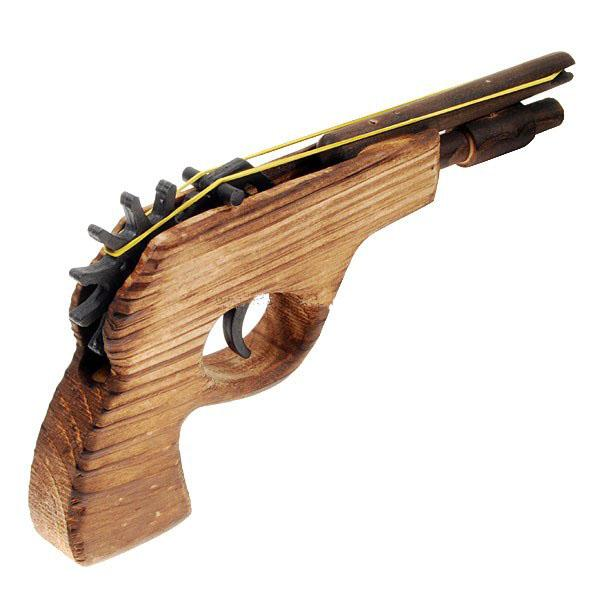
\includegraphics[scale=.45]{rubber-band-gun}
		\end{center}
	\subsection{Rotating Platform}
		1 motor will be controlled with proportional and integral controls (PID).  The joystick (described under 1.3 Turret Control) will allow user control over the turret's rotation. 
	\subsection{Turret Control}
		The rotating platform's angle will be determined via a wired joystick with a potentiometer.  The potentiometers are used to calculate the difference between the joystick and the platform angle of rotation (see code flowchart below).  An attached button will function as a remote trigger to fire the rubber band gun.
\newpage
\section{Schematics}
	\subsection{Potentiometer Control}
	\begin{figure}[!ht]
		\centering
		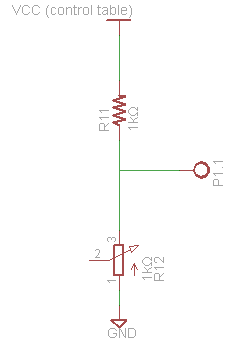
\includegraphics{potentiometer-control}
		\caption{Potentiometer Control.  The potentiometer has a linear taper.}
	\end{figure}
	\subsection{Button Control}
	\begin{figure}[!ht]
		\centering
		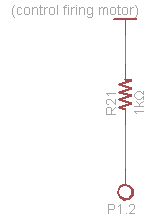
\includegraphics{button-control}
		\caption{Button Control}
	\end{figure}
	\subsection{Potentiometer Sensor}
	\begin{figure}[!ht]
		\centering
		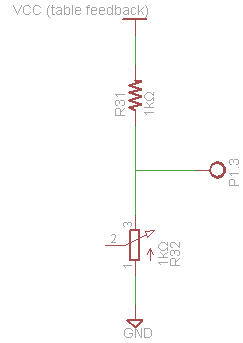
\includegraphics{potentiometer-sensor}
		\caption{Potentiometer Sensor.  The potentiometer has a linear taper.}
	\end{figure}
\newpage
	\subsection{Table Motor}
	\begin{figure}[!ht]
		\centering
		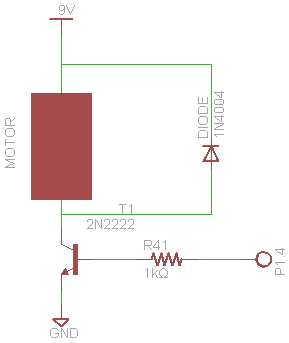
\includegraphics{table-motor}
		\caption{Table Motor}
	\end{figure}
	\subsection{Firing Motor}
	\begin{figure}[!ht]
		\centering
		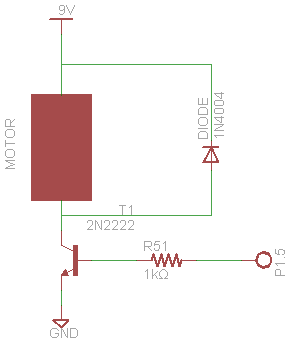
\includegraphics{firing-motor}
		\caption{Firing Motor}
	\end{figure}
\newpage
\section{Code Flowchart}
\bigskip
\begin{center}
	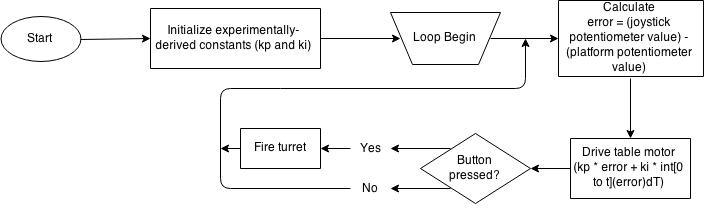
\includegraphics[width=7in]{group-turret-flowchart}
\end{center}
\end{document}